
% \textbf{Excel Sheet \textit{Gene-level RNA Processing} ZIP File \newline 
% \textit{RNA secondary structure of RNaseIII sites}}

Decay intermediates captured by full-length PacBio RNA sequencing: 5' erosion 0154/lap and 3' erosion 0178.

RNA isoform truncation categories: 25\% of the isoforms are complete; biased 3' intragenic.

Could be Exo 3' to 5' initiate RNA degradation, unstructured 3' end to facilitate exo 3' to 5' digestion
; without experiments verification

Proposed mechanism to explain biased RNA processing: lower copy numbers of tmRNA/SmpB prevent the activities of RNase R on trapped mRNAs;

Intragenic truncated RNA isoforms stronly suggests endo-cleavage: ATP synthase operon have RNase III cleavage at \textit{atpA} peripheral gene

% RNase III cleavages sites mapped to Syn1 by homology comparison with \textit{B. subtilis}

% \begin{itemize}
%     \item Eight genes mapped with RNA secondary structure and isoform support
% \end{itemize}

% RNase Y cleavage sites mapped to Syn1

\textit{Correlation protein localization and cleavage activities}

% How many high confidence endo-cleavage sites? Which part of operons?

\begin{figure}[H]
    \centering
    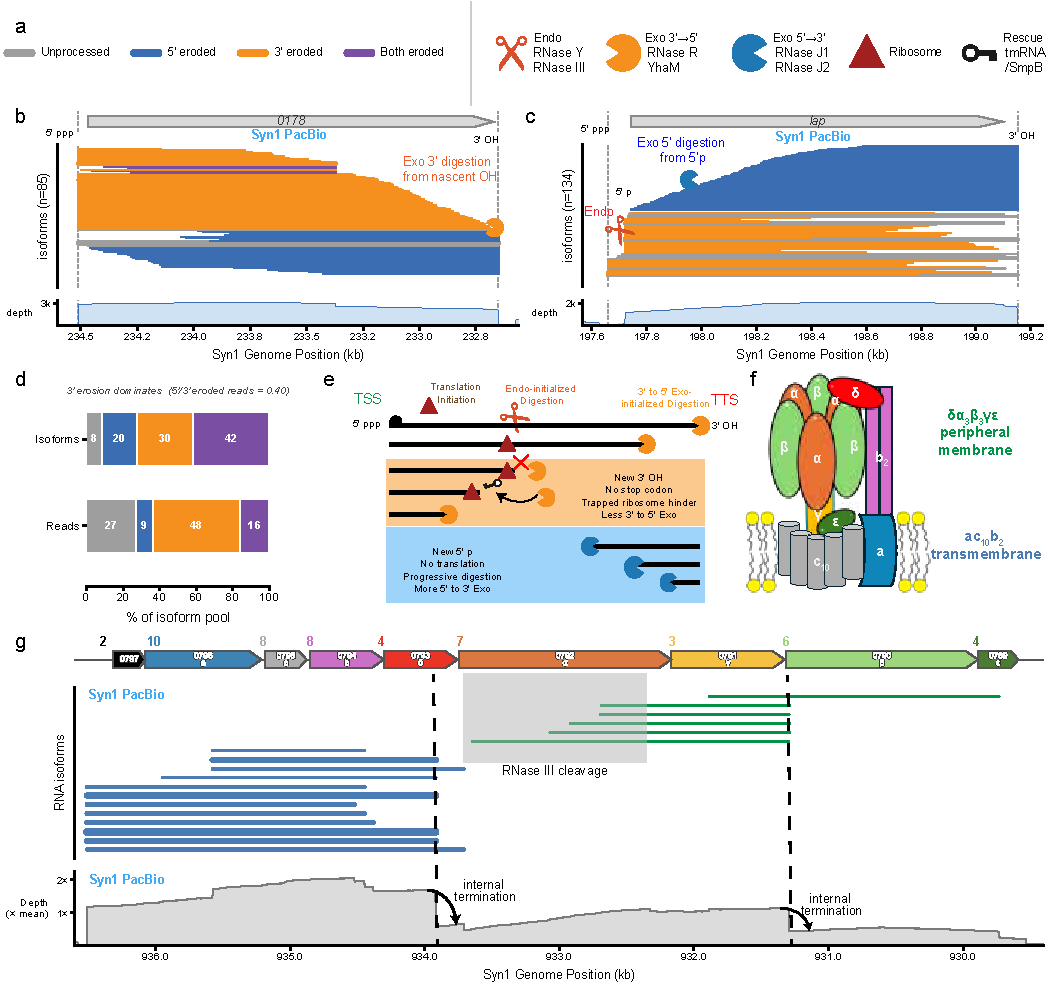
\includegraphics[width=1\linewidth]{figures/rnase.pdf}
    \caption{Caption}
    \label{fig:placeholder}
\end{figure}

\begin{table}[H]
\centering
\caption{Ribonucleases and \textit{trans}-Translation Rescue System in Syn1}
\begin{tabular}{C{2cm} C{3cm} C{2.0cm} C{3.0cm} C{4.0cm}}
\toprule
LocusNum & Gene Product & Abundance & Function & Activity Signature\\
\midrule

\textit{rnmV}/0003 & RNase M5 & 37 & Endo  & 5S rRNA\\
\textit{rny}/0359  & RNase Y & 70 & Endo &  ssRNA \newline degenerate features \\
\textit{rnc}/0418  & RNase III & 67 & Endo  & dsRNA \\

\hline

\textit{rnjB}/0257 & RNase J2 & 142 & Exo 5'$\rightarrow$3' & - \\
\textit{rnjA}/0600 & RNase J1 & 92 & Exo 5'$\rightarrow$3'  & 5' monophosphate \\
\textit{yhaM}/0437 & YhaM & 117 & Exo 3'$\rightarrow$5' & 3' OH \newline unstructured region \\
\textit{rnr}/0775  & RNase R & 36 & Exo 3'$\rightarrow$5' & 3' OH \newline unstructured region\\

\hline

\textit{ssrA}/0158 & tmRNA & 2.5\% of non-rRNA & Ribosome rescue & non-stop mRNA \\
\textit{smpB}/0776 & Small protein B & 14 & tmRNA cofactor & non-stop mRNA \\


\bottomrule
\label{tbl:rnase_syn1_syn3a}
\end{tabular}

\end{table}

\textbf{SI: Excel file Gene-level RNA Processing and Expression}

Sheet 1: RNA Processing mapped from B. subtilis